\subsection{MATLAB \hfill \normalsize(Release 2/2016)} \label{sec:MATLAB}

		\textit{\textbf{Encountered in: MAT\texttt{\_}SCI 405, 408}} 

MATLAB is a powerful computing environment that is commonly used by scientists and engineers of all disciplines for numerical simulation, data analysis, data visualization, hardware control, and creation of custom graphical user interfaces.

MATLAB's built-in functional utility is vast, and this is further supported by an active user community that interacts at the \href{https://www.mathworks.com/matlabcentral/fileexchange/}{MathWorks File Exchange}. There, you can find free user-generated content --- functions, applictions, examples, drivers, etc, that may prove useful in your coursework and research. 

MATLAB is installed on the computers in the Bodeen Laboratory and is also available for purchase by students (\$72/yr on campus, including VPN; \$130 off campus). Many research groups also have license subscriptions that can be utilized for your academic projects.

Below is a basic introduction to working with MATLAB. Some good resources and tutorials are linked below for further investigation. 

\subsubsection*{Suggested Resources:} 
		\begin{itemize}
			\item	\textit{Introduction to MATLAB}, David Houcque, Northwestern University (2005) \href{https://northwestern.box.com/s/13myp0an8snmmfjqfbx9gt1gbfrah0aj}{eReserve Link}\footnote{This is somewhat dated. I'm looking for a more up-to-date version.} %Is there a more recent version? This text is for MATLAB R2006.
			\item Ilya Mikhelson (Northwestern EECS) has developed a series of MATLAB tutorials and posted them on YouTube. Specifically useful tutorials are following
				\begin{enumerate}
					\item \href{https://www.youtube.com/watch?v=n1a4g2Z8Lb8&list=PL1ec5YBm_crwcmeR8pKB9shvnriE8UbFE&index=1}{MATLAB Script Tutorial}
					\item \href{https://www.youtube.com/watch?v=JE7I4Krj1PU&list=PL1ec5YBm_crwcmeR8pKB9shvnriE8UbFE&index=2}{MATLAB Indexing Tutorial}
					\item \href{https://www.youtube.com/watch?v=HfRv3NMV6Ys&list=PL1ec5YBm_crwcmeR8pKB9shvnriE8UbFE&index=3}{MATLAB Logical Expression Tutorial}
					\item \href{https://www.youtube.com/watch?v=HfRv3NMV6Ys&list=PL1ec5YBm_crwcmeR8pKB9shvnriE8UbFE&index=6}{MATLAB Subarray Tutorial}
					\item \href{https://www.youtube.com/watch?v=HfRv3NMV6Ys&list=PL1ec5YBm_crwcmeR8pKB9shvnriE8UbFE&index=7}{MATLAB Concatenation Tutorial}
					\item \href{https://www.youtube.com/watch?v=HfRv3NMV6Ys&list=PL1ec5YBm_crwcmeR8pKB9shvnriE8UbFE&index=8}{MATLAB Variable Declaration Tutorial}
					\item \href{https://www.youtube.com/watch?v=HfRv3NMV6Ys&list=PL1ec5YBm_crwcmeR8pKB9shvnriE8UbFE&index=10}{MATLAB For Loops Tutorial} and \href{https://www.youtube.com/watch?v=HfRv3NMV6Ys&list=PL1ec5YBm_crwcmeR8pKB9shvnriE8UbFE&index=11}{MATLAB While Loops Tutorial}
					\item \href{https://www.youtube.com/watch?v=HfRv3NMV6Ys&list=PL1ec5YBm_crwcmeR8pKB9shvnriE8UbFE&index=12}{MATLAB Function Tutorial}
					\item \href{https://www.youtube.com/watch?v=HfRv3NMV6Ys&list=PL1ec5YBm_crwcmeR8pKB9shvnriE8UbFE&index=13}{MATLAB Debugging Tutorial}
				\end{enumerate}
			\end{itemize}

\subsubsection{Interfacing with MATLAB}

When a user first opens MATLAB (this guide is written for the current version of MATLAB as of 2/2017: MATLAB 9.1) as shown in Fig. \ref{fig:MatlabApplication} with various sub-windows visible.

\begin{figure}[!b]%
	\centering
	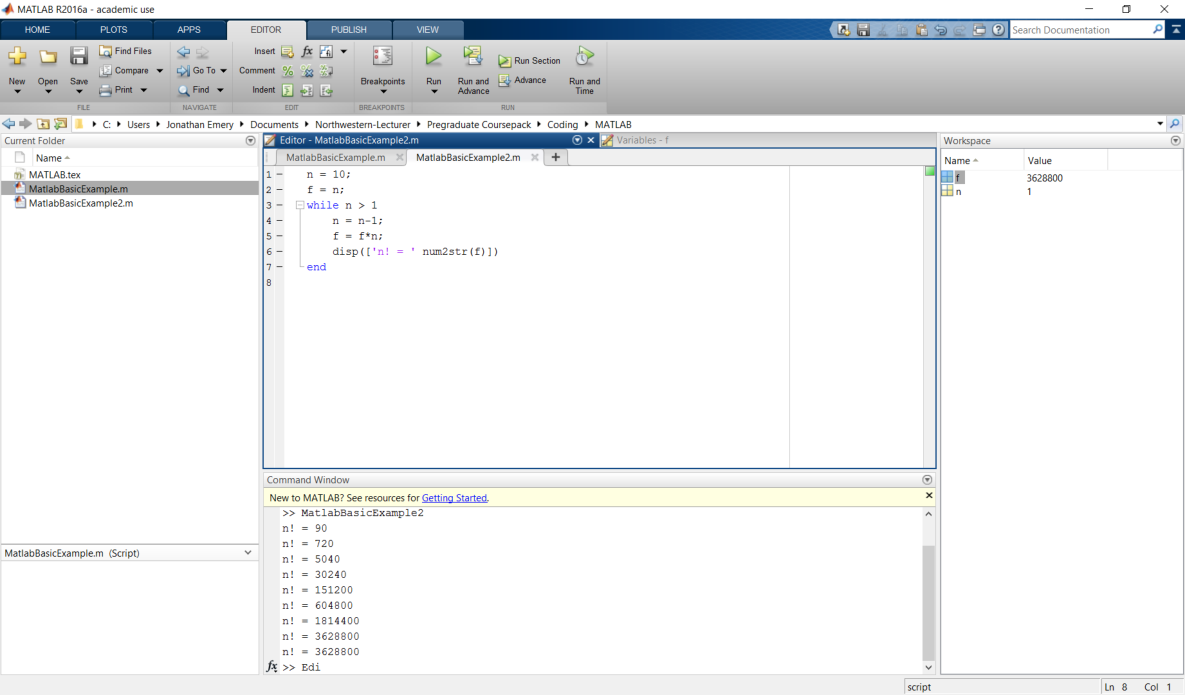
\includegraphics[width=0.8\columnwidth]{MatlabApplication}%
	\caption{The MATLAB user interface, MATLAB 9.1.}%
	\label{fig:MatlabApplication}%
\end{figure}

	\begin{itemize}[align=left]
		\item [\textbf{Current Folder:}] This window (at the far left) shows the files that are present in your current directory. This can be changed by navigating to a different directory, shown in the field directly above the windows.
		\item [\textbf{Command Window:}] This window allows you to directly input commands in a command-line format. This is useful for simple, quick calculations and plots. For more extensive calculations you will need to write a script in the Editor.
		\item [\textbf{Editor:}] You will use this space to write and edit your code. While you can, in principle, edit MATLAB code in \emph{any} text editor, MATLAB's editor is ideally suited to editing its own code and provides utilities that facilitate your scripting, including color-coded syntax, debugging options, and script comparison tools. These scripts are saved as so-called ``m-files'', with extension \verb|.m|.
		\item [\textbf{Workspace:}] The workspace contains data structures (scalars, vectors, matrices, tensors, and structure/cell arrays) that are created during your session. The woskpace provides you with at-a-glance information about, for example the data name, value, class, size, and statistics. You can view the data values by double-clicking on the data icon. This will open a sub-tab within the editor window which allows you to easily access and edit your data.
	\end{itemize}


\subsubsection{Basic Commands and Arithmetic Syntax}

MATLAB possess its own scripting language and possess unique syntax. Below we list a selection --- and some examples --- of the most basic MATLAB commands. When appropriate, you can copy these examples directly into the command line or m-file and execute. The output will appear in the Command Window. This list is sourced from a document compiled from the $\Eta \Kappa \Nu$ society at the University of Minnesota. The full source can be found  \href{http://www.hkn.umn.edu/resources/files/matlab/MatlabCommands.pdf}{here}.

When operating in the command window there are a useful set of session managing commands that will streamline your workflow. These are listed in Tab. \ref{tab:SessionMATLABSyntax}. 

\begin{table}[b]%
	\centering
	\begin{tabularx}{4.1in}{lcc}
	\toprule
		Description & Syntax & Example\\
	\midrule
		 \multicolumn{3}{c}{Session Management Operations}\\
	\midrule
		Clear command window & {\lstinline[style=Matlab-editor]!clc!} &  \\
		Clear variables & {\lstinline[style=Matlab-editor]!clear!} & \\
		Returns help page & {\lstinline[style=Matlab-editor]!help!} &  {\lstinline[style=Matlab-editor]!help circshift!} \\
		Set global variable & {\lstinline[style=Matlab-editor]!global!} &  {\lstinline[style=Matlab-editor]!global x!} \\
		Quit MATLAB & {\lstinline[style=Matlab-editor]!quit!} &  \\
		Display/use most resent answer & {\lstinline[style=Matlab-editor]!ans!} &  {\lstinline[style=Matlab-editor]!ans+2!}\\
	\midrule
	\end{tabularx}
	\caption{Syntax for managing MATLAB sessions.}
	\label{tab:SessionMATLABSyntax}
\end{table}

Simple arithmetic operations and special variables are tabulated in Fig. \ref{tab:ArthmeticMATLABSyntax}.

\begin{table}%
	\centering
	\begin{tabularx}{3.2in}{lcc}
	\toprule
		Description & Syntax & Example \\
	\midrule
		 \multicolumn{3}{c}{Arithmetic Operations and Special Variables}\\
	\midrule
		Addition & {\lstinline[style=Matlab-editor]!+!} & {\lstinline[style=Matlab-editor]!1+1!} \\
		Subtraction & {\lstinline[style=Matlab-editor]!-!} & {\lstinline[style=Matlab-editor]!1-1!} \\
		Multiplication & {\lstinline[style=Matlab-editor]!*!} & {\lstinline[style=Matlab-editor]!2*1!} \\
		Right-Hand Division & {\lstinline[style=Matlab-editor]!/!} & {\lstinline[style=Matlab-editor]!1/2!} \\
		Left-Hand Division & {\lstinline[style=Matlab-editor]!\\!} & {\lstinline[style=Matlab-editor]!1\\2!} \\
		Exponentiation & {\lstinline[style=Matlab-editor]!^!} & {\lstinline[style=Matlab-editor]!e^2!} \\
		Assignment & {\lstinline[style=Matlab-editor]!=!} & {\lstinline[style=Matlab-editor]!a = 1!} \\
		Grouping & {\lstinline[style=Matlab-editor]!( )!} & {\lstinline[style=Matlab-editor]!2*(3+6)!} \\
		The number $\pi$ & {\lstinline[style=Matlab-editor]!pi!} & {\lstinline[style=Matlab-editor]!2*pi!} \\
		Imaginary number $\sqrt{-1}$ & {\lstinline[style=Matlab-editor]!i,j!} & {\lstinline[style=Matlab-editor]!1 + 3i!} \\
		Infinity & {\lstinline[style=Matlab-editor]!Inf!} & {\lstinline[style=Matlab-editor]!1/0!} \\
		Not-a-Number & {\lstinline[style=Matlab-editor]!NaN!} & {\lstinline[style=Matlab-editor]!Inf/Inf!} \\
	\midrule
	\end{tabularx}
	\caption{Arithmetic MATLAB syntax and special variables.}
	\label{tab:ArthmeticMATLABSyntax}
\end{table}

\subsubsection{Matrix Notation and Operations}

MATLAB is recognized for its strength in writing, representing, and operating on arrays. The construction of matrices in MATLAB is straightforward --- examples are shown in Tab. \ref{tab:ArrayMATLABSyntax}.

When entering the example commands in the command line, a matrix-form output will be created. You can also see and edit these matrices by using the Workspace and accessing the Variable Spreadsheet.

\begin{table}[!b]%
	\centering
	\begin{tabularx}{5.6in}{lcc}
	\toprule
		Description & Syntax & Example \\
	\midrule
		 \multicolumn{3}{c}{Array Creation}\\
	\midrule
		Row Vector & {\lstinline[style=Matlab-editor]![. . .]!} & {\lstinline[style=Matlab-editor]!a = [1 2 3 4]!} \\
		Column Vector & {\lstinline[style=Matlab-editor]![. ; . ; .]!} & {\lstinline[style=Matlab-editor]!a = [1; 2; 3; 4]!} \\
		2 $\times$ 2 Matrix & {\lstinline[style=Matlab-editor]![. . ; . . ;]!} & {\lstinline[style=Matlab-editor]!a = [1 2; 3 4]!} \\
		Create $n \times m$ matrix  & \pbox{20em}{
		{\lstinline[style=Matlab-editor]!zeroes(n,m)!}\\
		{\lstinline[style=Matlab-editor]!ones(n,m)!}\\
		{\lstinline[style=Matlab-editor]!randi([-b,b],n,m)!}} &
		\pbox{20em}{
		{\lstinline[style=Matlab-editor]!zeroes(3,1)!}\\
		{\lstinline[style=Matlab-editor]!ones(3,5)!}\\
		{\lstinline[style=Matlab-editor]!rand([-5,5],4,4)!}}\\
	\midrule
		 \multicolumn{3}{c}{Accessing Matrix Elements}\\
	\midrule
		Access Row $i$, column $j$ of $A$ & {\lstinline[style=Matlab-editor]!A(i,j)!} & {\lstinline[style=Matlab-editor]!A(3,2)!} \\
		Access $i$\textsuperscript{th} row of $A$ & {\lstinline[style=Matlab-editor]!A(i,:)!} & {\lstinline[style=Matlab-editor]!A(1,:)!} \\
		Access $j$\textsuperscript{th} column of $A$ & {\lstinline[style=Matlab-editor]!A(:,j)!} & {\lstinline[style=Matlab-editor]!A(:,2)!} \\
		Access submatrix of $A$ & {\lstinline[style=Matlab-editor]!A([i1 i2],[j1, j2 ,3])!} & {\lstinline[style=Matlab-editor]!A([1 2], [1 2 4])!} \\
	\midrule
		 \multicolumn{3}{c}{Matrix Operations}\\
	\midrule
		Matrix Transpose & {\lstinline[style=Matlab-editor]!A'!} &  \\
		Matrix Inverse & {\lstinline[style=Matlab-editor]!inv(A)!} &  \\
		Matrix Multiplication & {\lstinline[style=Matlab-editor]!A*B!} &  \\
		Matrix Inverse Multiplication & {\lstinline[style=Matlab-editor]!A/B!} or {\lstinline[style=Matlab-editor]!A*inv(B)!} & \\
		Matrix Exponentiation to $n$ & {\lstinline[style=Matlab-editor]!A^n!} &  \\
		Matrix Cross-product & {\lstinline[style=Matlab-editor]!cross(A,B)!}  & \\
		Matrix Dot-product {\lstinline[style=Matlab-editor]!dot(A,B)!}  & \\
		Element-by-element operations & 	\pbox{20em}{
		{\lstinline[style=Matlab-editor]!A.*B!}\\
		{\lstinline[style=Matlab-editor]!A./B!}\\
		{\lstinline[style=Matlab-editor]!A.^n!}} & \\
		Return $n \times m$ size of A & {\lstinline[style=Matlab-editor]!size(A)!} &  \\
 		Concatenate column X onto A & {\lstinline[style=Matlab-editor]![A X]!} &  \\
		Concatenate row Y onto A & {\lstinline[style=Matlab-editor]![A; Y]!} &  \\
	\bottomrule
	\end{tabularx}
	\caption{MATLAB syntax for creating and operating on matrices. To test operations possesing A, B, X or Y you must first create those matrices.}
	\label{tab:ArrayMATLABSyntax}
\end{table}

\subsubsection{Creating and Using Functions}

MATLAB has a large number of built-in function that can provided with input and provide an output. Simple examples include {\lstinline[style=Matlab-editor]!cos(x)!} or {\lstinline[style=Matlab-editor]!sqrt(x)!}. When functions are called from script files they must be saved as individual files within the working directory (or a directory which has been added to the path). Example syntax for defining a ``Power'' function, which takes a input variable and outputs the computed result is shown below. This function can be called within a script to return variable {\lstinline[style=Matlab-editor]!p!}. The syntax here is: {\lstinline[style=Matlab-editor]!function [out1,out2, ..., outN] = myfun(in1,in2,in3, ..., inN)!}, where in1 ... inN are input variables and out1, ..., outN are output variables.

Autonomous functions are another way to define a user-supplied function without necessitating the creation of a new file when calling them in a script. These can be defined in the command line or in-line within the m-file. An example of use of an autonomous function is shown in Fig. \ref{subsubsection:mFile}.

				\lstinputlisting[
					style=Matlab-editor,
					basicstyle=\mlttfamily,
					escapechar=`,
					tabsize=2,
				]
				{./Coding/MATLAB/Power.m}

\newpage
\subsubsection{Control Flow and Iterative Loops}

A core component of any numerical calculation is the iterative loop that controls the simulation steps. These statements direct MATLAB to perform a certain calculation either \emph{while} certain conditions are true or \emph{for} certain a specific range/specific number of times. The general syntax here is {\lstinline[style=Matlab-editor]!disp!} 

				\lstinputlisting[
					style=Matlab-editor,
					basicstyle=\mlttfamily,
					escapechar=`,
					tabsize=2,
				]
				{./Coding/MATLAB/ForSyntax.m}
			
Below, we show an example of a {\lstinline[style=Matlab-editor]!for!} loop that simply displays the values over each iteration --- here from -2 ({\lstinline[style=Matlab-editor]!start!}) to 4 ({\lstinline[style=Matlab-editor]!finish!}) in steps of 0.5 ({\lstinline[style=Matlab-editor]!del!}). In place of the {\lstinline[style=Matlab-editor]!disp!} command you can place any command or series of commands, of course. 

				\lstinputlisting[
					style=Matlab-editor,
					basicstyle=\mlttfamily,
					escapechar=`,
					tabsize=2,
				]
				{./Coding/MATLAB/ForDisplay.m}

A {\lstinline[style=Matlab-editor]!while!} loop is shown below. This statement is useful when you are unsure about when the condition may become untrue (e.g. convergence criteria, etc.). The same example as shown above is show below, but now for the case which the index is less than or equal to the number of elements in the matrix. This job is more suitable for a {\lstinline[style=Matlab-editor]!for!} loop, but we show it below using a {\lstinline[style=Matlab-editor]!while!} loop for comparison. 

				\lstinputlisting[
					style=Matlab-editor,
					basicstyle=\mlttfamily,
					escapechar=`,
					tabsize=2,
				]
				{./Coding/MATLAB/WhileDisplay.m}

\subsubsection{Basic Plotting} \label{subsubsection:BasicPlotting}

You will inevitably want to visualize your data or computational results. MATLAB has a variety of tools to facility this. There are many, many options to plot data. Below we show a simple 2D plot that has some plotting options defined including axis ranges and labels.

The plot command {\lstinline[style=Matlab-editor]!mesh!} renders a wireframe figure of a scaled $sinc$ function with $Z$ values plotted with color. Thre sult is shown in Fig. \ref{fig:SincPlot} $X$ and $Y$ values are vectors that describe the plane. The example below shows a full, annotated m-file in which the last section (the plot section) defines plotting options including {\lstinline[style=Matlab-editor]!axis!} for axis range and {\lstinline[style=Matlab-editor]!xlabel!} for axis labels. 
		
				\lstinputlisting[
					style=Matlab-editor,
					basicstyle=\mlttfamily,
					escapechar=`,
					tabsize=2,
				]
				{./Coding/MATLAB/mFileExample.m}
				
				
		\begin{figure}%
			\centering
			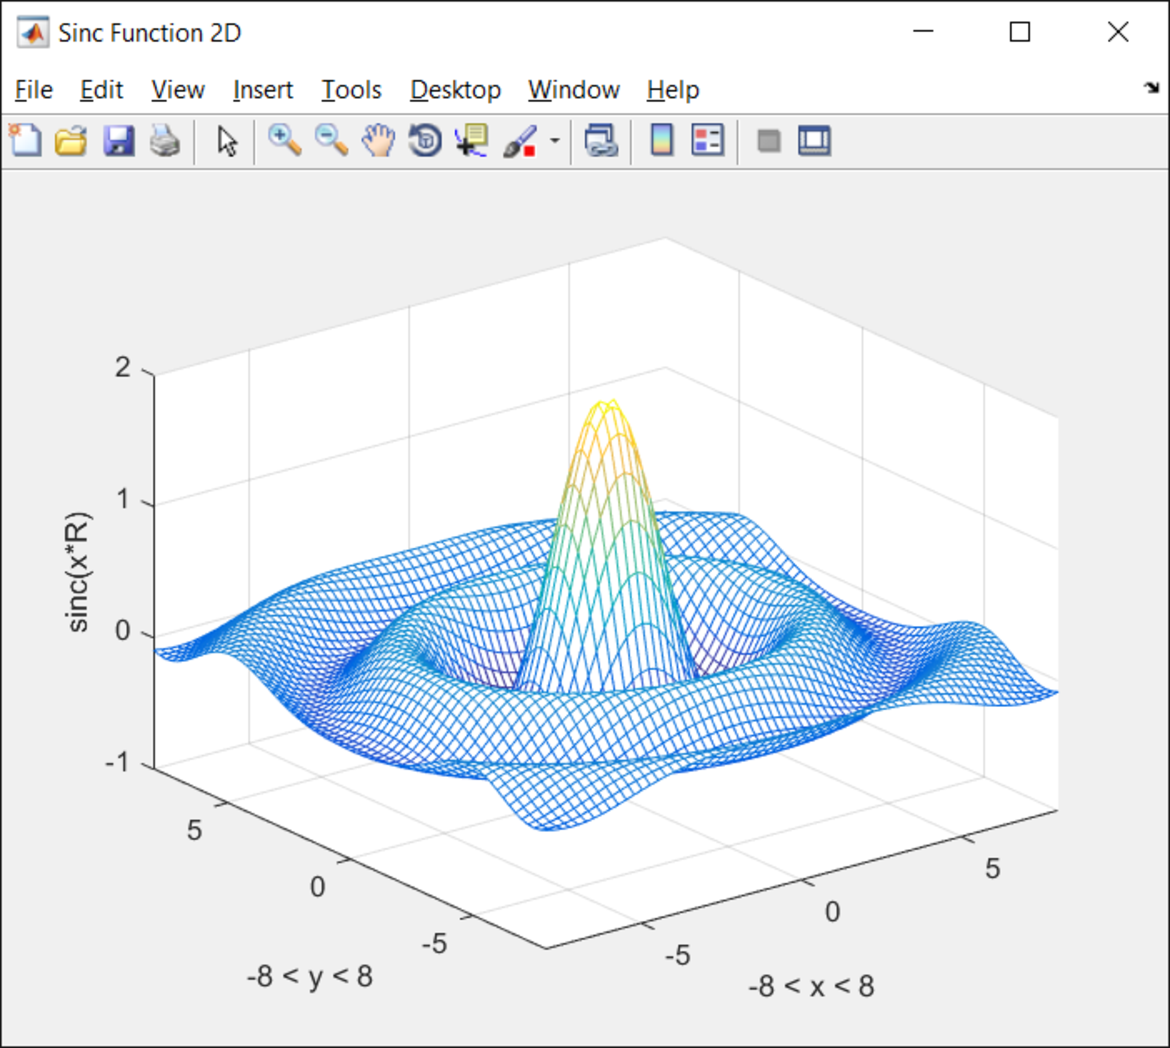
\includegraphics[width=0.5\columnwidth]{SincResult}%
			\caption{A meshplot of a sinc function.}%
			\label{fig:SincPlot}%
		\end{figure}	
								
	\subsubsection{Scripting and Debugging the m-file} \label{subsubsection:mFile}

Working with the command line is convenient for quickly accessing and working with data, or running scripts or creating custom functions. The examples above can be simply executed line-by-line in the the command window (although they were written as m-files), in doing so you will soon find, however, that it is much more convenient to write a script --- a series of commands --- in a m-file within the MATLAB editor. A script m-file operates simply by executing any commands listed in the file. A somewhat more advanced example is shown in Section \ref{subsubsection:BasicPlotting}. A very simple example for an m-file that uses the {\lstinline[style=Matlab-editor]!disp!} command to print ``Hello World''in the command window is shown below.

The example below also contains a commented-out \% preamble with file information as well as section breaks \%\% for organization. 

				\lstinputlisting[
					style=Matlab-editor,
					basicstyle=\mlttfamily,
					escapechar=`,
					tabsize=2,
				]
				{./Coding/MATLAB/HelloWorld.m}
				
Script m-files usually possess at least four sections (examples of all these sections, as well as a plotting section are shown in \ref{subsubsection:BasicPlotting}):

\begin{itemize}[align=left]
	\item [\textbf{The Preamble:}] This is where you will record pertinent notes about the file such as version history, authorship, licensing, or other comments. These are usually commented out with \% symbols. 
	\item [\textbf{Variable Declaration and Array Preallocation:}] After the preamble there is typically a section where you define the variables that will be used in the script\footnote{You can also create a MATALB {\lstinline[style=Matlab-editor]!function!} that accepts inputs and can be called from the command line.}. Preallocation of arrays with {\lstinline[style=Matlab-editor]!zeros(n,m)!} or {\lstinline[style=Matlab-editor]!ones(n,m)!} can greatly reduce the amount of memory consumed by MATLAB --- especially when arrays iteratively grow when the script is run.  
		\item [\textbf{Anonymous Function:}] Often, you will want to add a function that is not built into MATLAB syntax or that does not need its own program file. These functions are often added at the end the m-file and are accessed when the script is run.
	\item [\textbf{Main Script:}] This is where the calculations are performed and the data is saved or plotted.
\end{itemize}

MATLAB provides a number of interactive tools to simplify codeing and debugging. Useful tools exist in the editor ribbon, including insert of sections of functios (from a library) or indent and comment control. Arguably, the most valuable tool is the setting and handling of breakpoints. Breakpoints are especially useful when constructing loops because the calulations can be monitored step-by-step through the loop.

\begin{figure}[b!]%
	\centering
	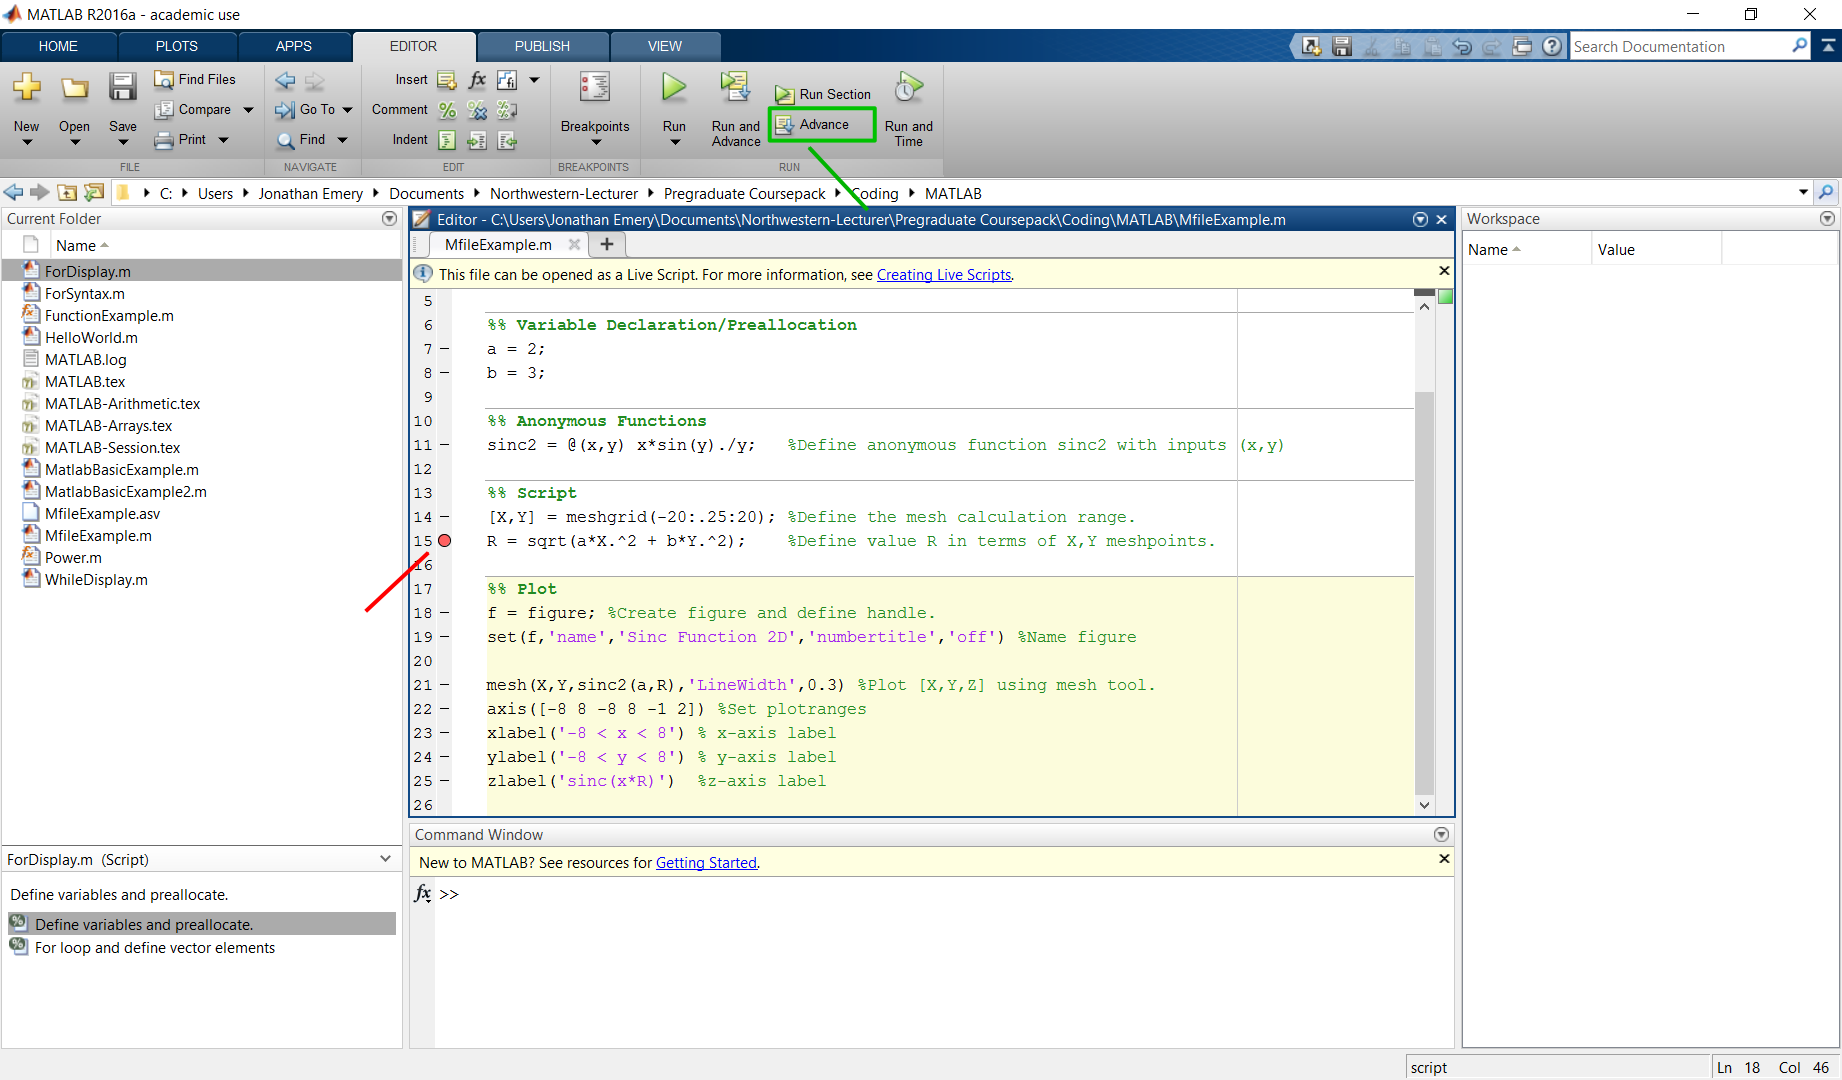
\includegraphics[width=0.7\columnwidth]{MATLABDebug}%
	\caption{Debugging MATLAB scripts.}%
	\label{fig:Breakpoint}%
\end{figure}

To set a breakpoint simply left click on the horizontal dash next to the line you would like to break at (indicated with a red arrow, Fig. \ref{fig:Breakpoint}). Run the code. Your script will stop at this point and you can investigate variable values. Then, you can advance the code to the next breakpoint (Fig. \ref{fig:Breakpoint}, green square). When in a loop this command will iterate the loop one step. When ready, you can use the breakpoints button to eliminate all breakpoints and run the code.



		